% SFT + DPO iterated training loop — poster figure
% Compile: tectonic loop_sft_dpo.tex
\documentclass[tikz,border=8pt]{standalone}
\usepackage{amssymb}
\usetikzlibrary{arrows.meta,positioning,fit,backgrounds,calc}
\renewcommand{\familydefault}{\sfdefault}

\definecolor{navy}{HTML}{16244F}
\definecolor{cardblue}{HTML}{EAF1FB}
\definecolor{borderblue}{HTML}{1A3D7C}
\definecolor{subgray}{HTML}{5A6A8A}
\definecolor{cardpurple}{HTML}{F6F0FB}
\definecolor{borderpurple}{HTML}{5E35B1}
\definecolor{textpurple}{HTML}{4A148C}
\definecolor{subpurple}{HTML}{6A4F8A}
\definecolor{cardred}{HTML}{FDF0EE}
\definecolor{borderred}{HTML}{C62828}
\definecolor{textred}{HTML}{B71C1C}
\definecolor{subred}{HTML}{A05252}
\definecolor{chipgreenbg}{HTML}{DCEDC8}
\definecolor{chipgreenfg}{HTML}{1B5E20}
\definecolor{chipgreenbd}{HTML}{2E7D32}
\definecolor{chipredbg}{HTML}{FFCDD2}

\begin{document}
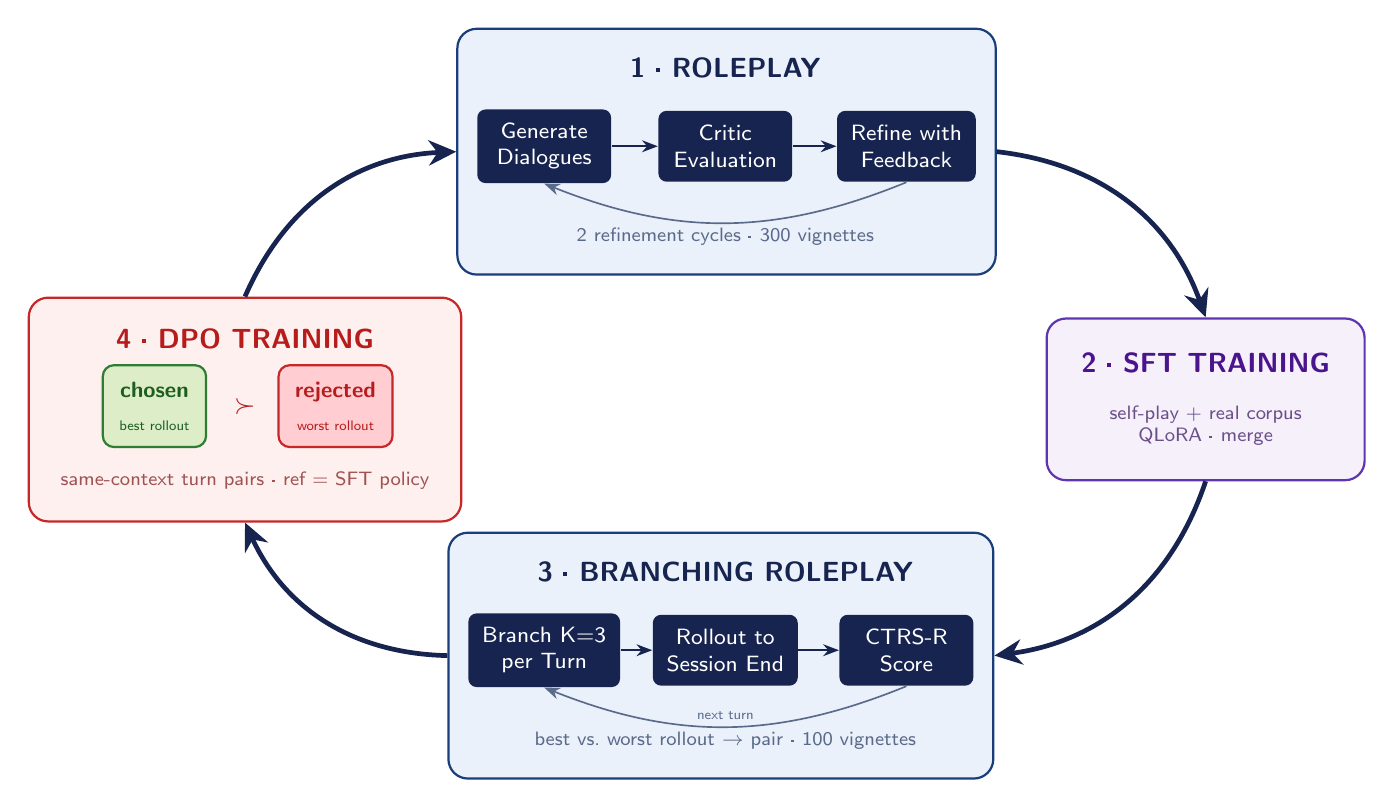
\begin{tikzpicture}[
  chip/.style={rounded corners=3pt, fill=navy, text=white, font=\footnotesize,
               align=center, inner sep=5pt, minimum height=9mm, minimum width=17mm},
  labelchip/.style={rounded corners=4pt, align=center, inner sep=6pt},
  chiparrow/.style={-{Stealth[length=2mm]}, navy, thick},
  loopback/.style={-{Stealth[length=2mm]}, subgray, semithick},
  ring/.style={-{Stealth[length=3.5mm,width=3.2mm]}, navy, line width=1.7pt},
  foot/.style={font=\scriptsize, text=subgray},
]

% ── Stage 1 · ROLEPLAY (top) ────────────────────────────────────────────
\begin{scope}[shift={(0,3.2)}]
  \node[chip] (s1a) at (-2.3,0) {Generate\\Dialogues};
  \node[chip] (s1b) at (0,0)    {Critic\\Evaluation};
  \node[chip] (s1c) at (2.3,0)  {Refine with\\Feedback};
  \draw[chiparrow] (s1a) -- (s1b);
  \draw[chiparrow] (s1b) -- (s1c);
  \draw[loopback] (s1c.south) to[bend left=22] (s1a.south);
  \node[font=\bfseries, text=navy] (s1t) at (0,1.0) {1 · ROLEPLAY};
  \node[foot] (s1f) at (0,-1.15) {2 refinement cycles · 300 vignettes};
  \begin{scope}[on background layer]
    \node[fit=(s1a)(s1c)(s1t)(s1f), rounded corners=7pt, fill=cardblue,
          draw=borderblue, thick, inner sep=7pt] (card1) {};
  \end{scope}
\end{scope}

% ── Stage 2 · SFT TRAINING (right) ──────────────────────────────────────
\begin{scope}[shift={(6.1,0)}]
  \node[font=\bfseries, text=textpurple] (s2t) at (0,0.45) {2 · SFT TRAINING};
  \node[font=\scriptsize, text=subpurple, align=center] (s2s) at (0,-0.35)
        {self-play + real corpus\\QLoRA · merge};
  \begin{scope}[on background layer]
    \node[fit=(s2t)(s2s), rounded corners=7pt, fill=cardpurple,
          draw=borderpurple, thick, inner sep=9pt] (card2) {};
  \end{scope}
\end{scope}

% ── Stage 3 · ROLEPLAY (bottom) ─────────────────────────────────────────
\begin{scope}[shift={(0,-3.2)}]
  \node[chip] (s3a) at (-2.3,0) {Branch K=3\\per Turn};
  \node[chip] (s3b) at (0,0)    {Rollout to\\Session End};
  \node[chip] (s3c) at (2.3,0)  {CTRS-R\\Score};
  \draw[chiparrow] (s3a) -- (s3b);
  \draw[chiparrow] (s3b) -- (s3c);
  \draw[loopback] (s3c.south) to[bend left=22]
      node[midway, above=-1pt, font=\tiny, text=subgray] {next turn} (s3a.south);
  \node[font=\bfseries, text=navy] (s3t) at (0,1.0) {3 · BRANCHING ROLEPLAY};
  \node[foot] (s3f) at (0,-1.15) {best vs.\ worst rollout $\rightarrow$ pair · 100 vignettes};
  \begin{scope}[on background layer]
    \node[fit=(s3a)(s3c)(s3t)(s3f), rounded corners=7pt, fill=cardblue,
          draw=borderblue, thick, inner sep=7pt] (card3) {};
  \end{scope}
\end{scope}

% ── Stage 4 · KTO TRAINING (left) ───────────────────────────────────────
\begin{scope}[shift={(-6.1,0)}]
  \node[font=\bfseries, text=textred] (s4t) at (0,0.75) {4 · DPO TRAINING};
  \node[labelchip, fill=chipgreenbg, draw=chipgreenbd, thick] (s4a) at (-1.15,-0.1)
        {\textcolor{chipgreenfg}{\footnotesize\textbf{chosen}}\\
         \textcolor{chipgreenfg}{\tiny best rollout}};
  \node[labelchip, fill=chipredbg, draw=borderred, thick] (s4b) at (1.15,-0.1)
        {\textcolor{textred}{\footnotesize\textbf{rejected}}\\
         \textcolor{textred}{\tiny worst rollout}};
  \node[font=\normalsize, text=textred] at (0,-0.1) {$\succ$};
  \node[font=\scriptsize, text=subred] (s4f) at (0,-1.05)
        {same-context turn pairs · ref = SFT policy};
  \begin{scope}[on background layer]
    \node[fit=(s4t)(s4a)(s4b)(s4f), rounded corners=7pt, fill=cardred,
          draw=borderred, thick, inner sep=8pt] (card4) {};
  \end{scope}
\end{scope}

% ── Clockwise ring ──────────────────────────────────────────────────────
\draw[ring] (card1.east) to[bend left=32] (card2.north);
\draw[ring] (card2.south) to[bend left=32] (card3.east);
\draw[ring] (card3.west) to[bend left=32] (card4.south);
\draw[ring] (card4.north) to[bend left=32] (card1.west);

\end{tikzpicture}
\end{document}
